\begin{frame}{$d(K^-, n)"\pi^{\mp}\Sigma^{\pm}"$ Cross Section}
  \begin{tabular}{cc}
    \begin{minipage}{0.5\hsize}
      \begin{figure}
        \textcolor{red}{$d(K^-, n)"\pi^-\Sigma^+$}
        \textcolor{blue}{$d(K^-, n)"\pi^+\Sigma^-$}
        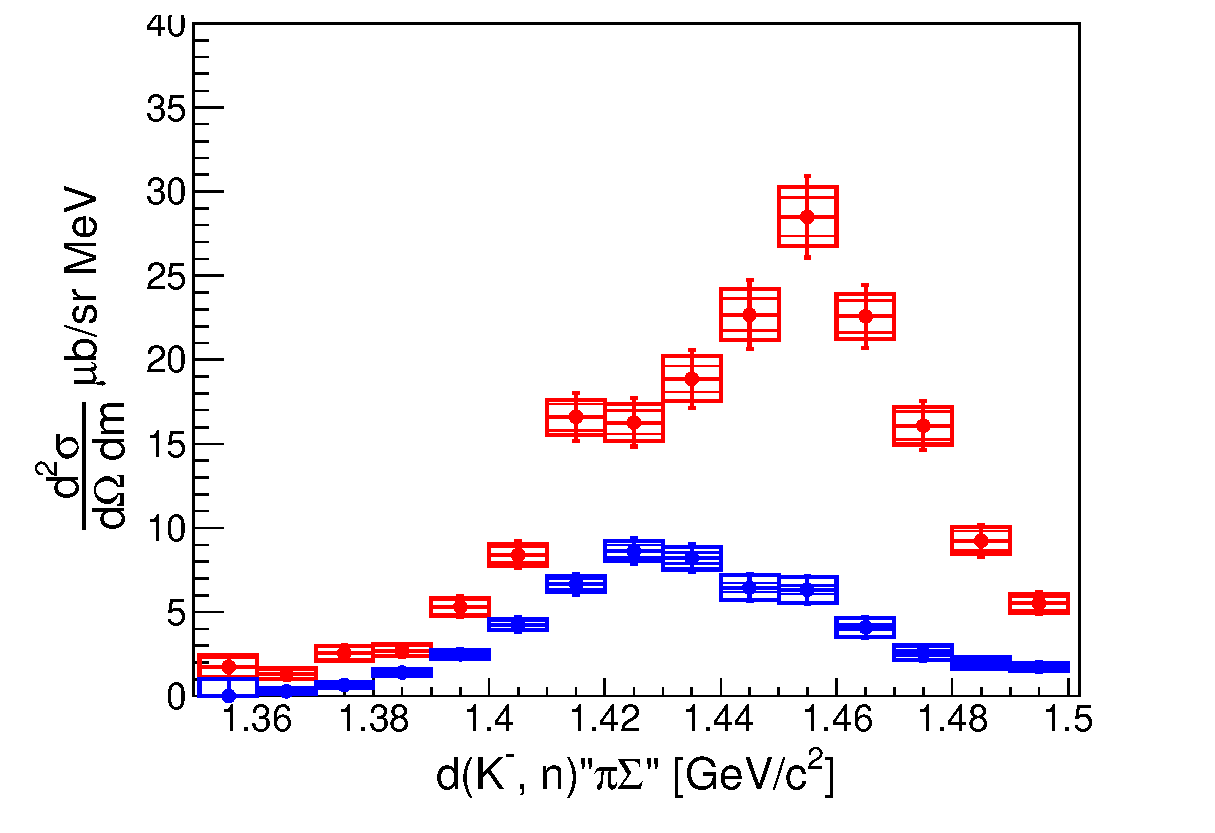
\includegraphics[width=6cm]{../pic/Run78/K0_ts_L1520/ChargeCS_after.eps}
      \end{figure}
    \end{minipage}

    \begin{minipage}{0.5\hsize}
      \begin{figure}
        Average of $d(K^-, n)"\pi^{\mp}\Sigma^{\pm}"$
        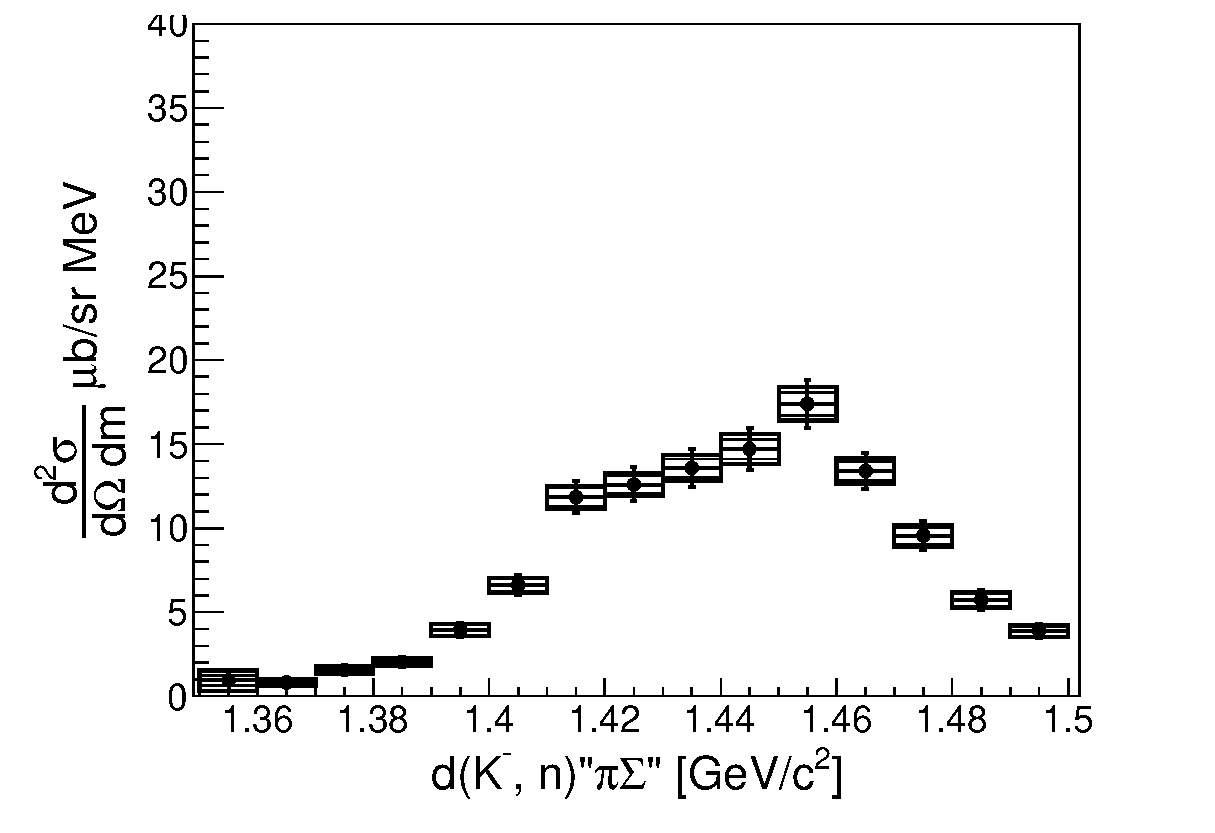
\includegraphics[width=6cm]{../pic/Run78/K0_ts_L1520/ChargeCS_ave_after.eps}
      \end{figure}
    \end{minipage}
  \end{tabular}
  \centering
  \scriptsize
  Inner boxs indicate statisical errors, outer boxs indicate statisical and fitting errors.\\
  Error bars include scaling factor which is common weight for all bins.

  \vspace{3mm}
  \small
  Large scattering amplitude was observed even in the $\bar{K}N$ threshold.
\end{frame}
